%\documentclass[10pt,twocolumn,letterpaper,draft]{article}
\documentclass[10pt,letterpaper]{ctexart}

\usepackage{cvpr}
\usepackage{graphicx}
\usepackage{wrapfig}
\usepackage{amsmath}
\newtheorem{myDef}{Definition}
\newtheorem{myTheo}{Theorem}

\usepackage{amssymb}
\usepackage{booktabs}
\usepackage{subfigure}
\usepackage{algorithm}
\usepackage{algorithmicx}
\usepackage{algpseudocode}
\usepackage{pythonhighlight}
\usepackage{xcolor}
\usepackage{listings}

\lstset{language=C++,
    basicstyle=\ttfamily,
    frame=single,
    keywordstyle=\color{blue}\ttfamily,
    stringstyle=\color{magenta}\ttfamily,
    commentstyle=\color{green}\ttfamily,
    morecomment=[l][\color{magenta}]{\#},
    morekeywords={*,uint_fast64_t}
}

\renewcommand{\labelenumi}{\alph{enumi}.} % Make numbering in the enumerate environment by letter rather than number (e.g. section 6)
\floatname{algorithm}{算法}
\renewcommand{\algorithmicrequire}{\textbf{输入:}}
\renewcommand{\algorithmicensure}{\textbf{输出:}}
\renewcommand{\lstlistingname}{代码清单}

\usepackage{enumitem}
\setenumerate[1]{itemsep=0pt,partopsep=0pt,parsep=\parskip,topsep=5pt}
\setitemize[1]{itemsep=0pt,partopsep=0pt,parsep=\parskip,topsep=5pt}
\setdescription{itemsep=0pt,partopsep=0pt,parsep=\parskip,topsep=5pt}

% Include other packages here, before hyperref.

% If you comment hyperref and then uncomment it, you should delete
% egpaper.aux before re-running latex.  (Or just hit 'q' on the first latex
% run, let it finish, and you should be clear).
\usepackage[pagebackref=true,breaklinks=true,letterpaper=true,colorlinks,bookmarks=false]{hyperref}


\cvprfinalcopy % *** Uncomment this line for the final submission

\def\cvprPaperID{159} % *** Enter the CVPR Paper ID here
\def\httilde{\mbox{\tt\raisebox{-.5ex}{\symbol{126}}}}

\newcommand{\mypara}[1]{\paragraph{#1.}}

\graphicspath{{figures/}}

% Pages are numbered in submission mode, and unnumbered in camera-ready
%\ifcvprfinal\pagestyle{empty}\fi
\setcounter{page}{1}


%\begin{CJK*}{GBK}{song}

\newcommand{\figref}[1]{图\ref{#1}}
\newcommand{\tabref}[1]{表\ref{#1}}
\newcommand{\equref}[1]{式\ref{#1}}
\newcommand{\secref}[1]{第\ref{#1}节}

\ctexset{
  section={
          name={,、},
          number={\chinese{section}},
          format={\heiti},
          beforeskip={0.1ex},
          afterskip={0.1ex},
          aftername={\nobreak},
          indent={\parindent},
          },
}
\usepackage{zhnumber}

\newcommand\zhsubsec[1]{{% 中文小节
\bfseries{
\stepcounter{subsection}(\zhnum{subsection}){#1}}
\vspace{0.1pt}%
}}

%%%%%%%%% TITLE

\begin{document}
\pagestyle{plain}
\title{
    \begin{center}
        \phantom{Start!}
    	  \vspace{2cm}
        \center{\zihao{1} 中山大学数据科学与计算机学院}
        \center{\zihao{2} 计算机科学与技术专业-人工智能}
        \center{\zihao{2} 本科生实验报告}
        \center{(2018-2019学年秋季学期)}
    \end{center}
}
\maketitle

\begin{center}
    \setlength{\baselineskip}{40pt}
    \vspace{1cm}
    \zihao{-2}
    \center{
        \begin{tabular}{cc}
      	学\qquad 号:& \underline{~~~~~~16337113~~~~~~}  \\
      	姓\qquad 名:& \underline{~~~~~~~劳马东~~~~~~~}  \\
        教学班级:   & \underline{~~~~~教务2班~~~~~}  \\
      	专\qquad 业:& \underline{~~~~~~~~~超算~~~~~~~~}  \\
      	\end{tabular}
    }
\end{center}
\pagebreak

%%%%%%%%% BODY TEXT %%%%%%%%%%%%%%%%%%%%%%%%%%%%%%%%%%%%%%%%
\section{实验题目}
使用backtracking和forward-checking求解N皇后问题,要求:
\begin{itemize}[itemindent=1.5em]
  \item 报告中需要包含对两个算法的原理解释;
  \item 需要包含两种方法在性能上的对比和分析;
\end{itemize}

\section{实验内容}
\zhsubsec{算法原理}
\begin{enumerate}[itemindent=2em,label=\arabic*、]
  \item N皇后问题的CSP定义
  \par \qquad 将N个皇后放置在$N \times N$的棋盘上,使得对于任意两个皇后,它们不在同一行、
  不在同一列、不在同一对角线上。\figref{fig:8-queens}是8皇后问题的一个例子。
  \begin{figure}[H]
    \centering
    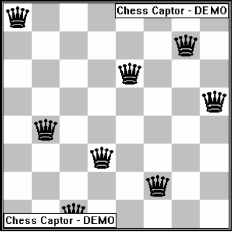
\includegraphics[width=0.2\textwidth]{N-queen.PNG}
    \caption{8皇后问题-Demo}
    \label{fig:8-queens}
  \end{figure}
  \begin{enumerate}[itemindent=2em,label=(\arabic*)]
    \item 变量集合
    \par \qquad N个皇后分别编号为0、1、2...N-1。如\figref{fig:8-queens}的8个皇后从上
    到下分别编号为0、1、2...6、7;
    \item 变量的值域
    \par \qquad $Q_i$表示第$i$个皇后的列号,则$Q_i \in [0, N)$。如\figref{fig:8-queens}
    每个皇后列号的取值范围为$\{0, 1, 2, 3, 4, 5, 6, 7\}$;
    \item 约束集
      \begin{itemize}[itemindent=2em]
        \item 列:$\forall\ i \neq j,\ Q_i \neq Q_j$
        \item 对角线:$\forall\ i \neq j,\ abs(Q_i - Q_j) \neq abs(i - j)$.
      \end{itemize}
      \par \qquad \figref{fig:8-queens}中8个皇后的列号分别为$Q_0=0$、$Q_1=6$、$Q_2=4$、
        $Q_3=7$、$Q_4=1$、$Q_5=3$、$Q_6=5$、$Q_7=2$。
  \end{enumerate}
  \item backtracking
  \par \qquad 回溯思想简单而言就是“一条路走到黑,不撞南墙不回头”,在解决问题时不断尝试值域中的每个取值,往下
  递归直到可以确定不可能补全成正确解时放弃搜索,回溯并选择值域中的下一个值。算法的整体流程如下:
  \begin{enumerate}[itemindent=2em,label=(\arabic*)]
    \item 如果所有的变量都被赋值了,算法结束。
    \item 否则选择一个未赋值的变量$Q_i$;
    \item 在$Q_i$的值域中选择一个值$x$,测试$Q_i=x$是否满足约束集,满足则回到步骤(1)。
    如果$Q_i$的所有取值都不满足约束,以搜索失败回溯。
  \end{enumerate}

    \par \qquad \figref{fig:4-queens}是用backtracking算法求解4皇后问题的过程,黑色表示当前可
    放置(即满足约束)的位置,蓝色是不可放置的位置。大体过程如下:
    \begin{itemize}[itemindent=2em]
      \item $Q_0$=0,无冲突;
      \item $Q_1$=0,与$Q_0$违反列约束;$Q_1$=1,与$Q_0$违反对角线约束;$Q_1$=2;
      \item $Q_2$=0,与$Q_0$违反列约束;$Q_2$=1或3,与$Q_1$违反对角线约束;$Q_2$=2,与$Q_1$违反列约束;
      无解,回溯到$Q_1$;
      \item $Q_1$=3,无冲突;
      \item 以类似的过程继续,在右下角找到了一个解。
    \end{itemize}
    在第二层,Q0
    \begin{figure}[H]
      \centering
      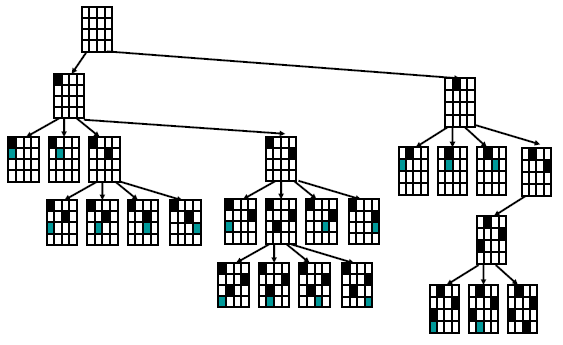
\includegraphics[width=0.55\textwidth]{4-queen.PNG}
      \caption{4皇后问题backtracking求解}
      \label{fig:4-queens}
    \end{figure}

    \begin{algorithm}
      \caption{backtracking搜索}
        \begin{algorithmic}[1] %每行显示行号
          \Require $Assigned$:N个皇后的赋值状态,$Column$:N个皇后的列号
            \Function {backtracking}{$Assigned, Column$}
              \If {all variables assigned}
                \State print all value of each variable
                \State \Return for more solutions \textbf{or} 
                \textbf{exit} for only one solution
              \Else
                \State {$V \gets$ PickUnassignedVariable()}
                \State $Assigned[V] \gets$ TRUE
                \For{\textbf{each} $v \in$ Domain($V$)}
                  \State $Column[V] \gets v$
                  \If {CheckConstraint() == TRUE}
                    \State backtracking($level + 1$)
                  \EndIf
                \EndFor
                \State $Assigned[V] \gets$ FALSE
                \State \Return
              \EndIf
            \EndFunction
        \end{algorithmic}
    \end{algorithm}
    
  \newpage
  \item forward-checking
  \par \qquad backtracking的问题在于,(1)一个皇后的列号确定之后,不对其他皇后的值域做更新,
  实际上可以利用皇后之间的约束关系简化其他皇后的值域;(2)只有“撞了南墙才回头”,给所有皇后尽可能
  地赋值后,才知道是否找到解。
  \par \qquad forward-checking是一种约束传播(Constraint Propagation)算法,在算法
  的每一步都“向前看”,将当前变量的赋值结果“传播”到其他还没有赋值的变量,更新它们的值域,
  从而当某个变量不可取值时提前回溯。
  \par \qquad 算法\ref{algo:fc}是该过程的伪代码,其中大部分与backtracking相同,增加了两个过程:一
  是当前变量赋值($Column[V]=v$)后,更新未赋值皇后的可取值范围($updateDomain$),并在{\color{red}回溯时恢复更新前
  的值域};二是判断某个被更新的值域是否为空,为空则说明$Column$现在的取值方式找不到解,回溯。

  \begin{algorithm}
    \caption{forward-checking搜索}
    \label{algo:fc}
      \begin{algorithmic}[1] %每行显示行号
        \Require $Assigned$:N个皇后的赋值状态,$Column$:N个皇后的列号, $CurDom$:N个皇后当前值域
          \Function {forward-checking}{$Assigned, Column, CurDom$}
            \If {all variables assigned}
              \State print all value of each variable
              \State \Return for more solutions \textbf{or} 
              \textbf{exit} for only one solution
            \Else
              \State {$V \gets$ PickUnassignedVariable()}
              \State $Assigned[V] \gets$ TRUE
              \For{\textbf{each} $v \in CurDom[V]$}
                \State $Column[V] \gets v$
                \State $DWO \gets$ updateDomain($CurDom, V, v, Assigned$)
                \If {$DWO$ happen}
                  \State \Return DWO
                \Else
                  \State forward-checking($Assigned, Column, CurDom$)
                \EndIf
                \State Restore($CurDomain, V, v, Assigned$)
              \EndFor
              \State $Assigned[V] \gets$ FALSE
              
            \EndIf
          \EndFunction
      \end{algorithmic}
  \end{algorithm}

    % \begin{figure}[H]
    % \centering
    % \subfigure[$Minimax$搜索例子]{
    % 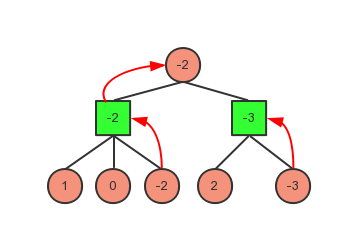
\includegraphics[width=0.4\textwidth]{minimax-example.png}
    % \label{fig:minimax-example}}
    % \subfigure[$\alpha \beta$剪枝例子1]{
    % 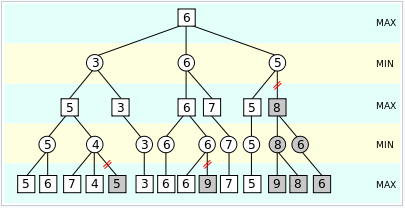
\includegraphics[width=0.5\textwidth]{ab-1.png}
    % \label{fig:alphabeta-example1}}
    % \end{figure}
\end{enumerate}

\newpage
\section{关键代码}
\begin{enumerate}[itemindent=2em,label=\arabic*、]
\item backtracking
\begin{python}
def n_queens_backtracking(chess_board, row=0):
    n = chess_board.shape[1]
    if row == n:    # n个皇后都被赋值了
        print(board)
        return 1    # 找到一个解
    else:
        cnt = 0
        for i in range(n):    # 皇后列号Qk的值域是[0, n)
            if csp(chess_board, (row, i)):  # Qk=i满足约束
                # 将皇后防放置在棋盘上
                chess_board[row][i] = 1
                # 往下递归,选择第row+1个皇后
                cnt += n_queens_backtracking(chess_board, row + 1)
                # 回溯,恢复棋盘状态
                chess_board[row][i] = 0
        return cnt
\end{python}

\item forward-checking值域更新
\begin{python}
for x in curdom_copy:
    restore = []     # 用于后面恢复值域
    ...
    for i in range(min_dom_index + 1, n):   # 所有未更新皇后在[min_dom_index + 1, n)
        other_queen_id, domain = domains[i]   # domains存了皇后id和它的列值域set
        restore.append(set())
        if x in domain:     # 同一列
            restore[-1].add(x)    # 被删除的元素放入restore
            domain.remove(x)
        for j in domain.copy():   # 同一对角线
            if abs(j - x) == abs(other_queen_id - queen_id):
                restore[-1].add(j)
                domain.remove(j)
        ...
\end{python}

\newpage
\item MRV选择变量
\begin{python}
for x in curdom_copy:
    ...
    min_dom_size = float('inf')
    min_dom_i = None
    # 找出被更新值域中,取值个数最少的一个
    for i in range(min_dom_index + 1, n):
        ...
        length = len(domain)
        if length < min_remain:
            min_dom_size = length
            min_dom_i = i
    # min_dom_size为0说明发生DWO
    if min_dom_i is not None and min_dom_size != 0:
        swap(domains, min_dom_index + 1, min_dom_i)
        cnt += n_queens_fc(board, index + 1, cnt + 1, domains)
\end{python}

\item forward-checking值域恢复
\begin{python}
if min_dom_i is not None and min_dom_size != 0:
    swap(domains, min_dom_index + 1, min_dom_i)
for j, d in enumerate(restore):
    domains[min_dom_index + j + 1][1].update(d)
\end{python}

\end{enumerate}

\section{实验结果及分析}
实验中测试了10皇后和12皇后问题,统计找出问题的所有解的运行时间,如\tabref{tab:time}。
10皇后问题解的个数为724个,使用backtracking算法时,需要6.39秒找出所有解,而使用forward-checking
只需0.23秒,只有backtracking时间的$\frac{1}{28}$左右;12皇后问题解的个数为14200,forward-checking
算法只有backtracking算法的$\frac{3.70}{231.03}\approx \frac{1}{62.4}$,更突显了forward-checking算法
的优越性。
\begin{table}[!htbp]
  \centering
  \begin{tabular}{cccc}
    \toprule  
    n& 解个数& backtracking时间/s& forward-checking时间/s\\
    \midrule  
    10& 724& 6.39& 0.23\\
    12& 14200& 231.03& 3.70\\
    \bottomrule 
  \end{tabular}
  \caption{算法运行时间}
  \label{tab:time}
\end{table}
\par 从定性的角度分析,backtracking算法每次递归都认为皇后的值域是[0, N),并且对每个值都运行一遍约束检测;
而forward-checking算法每个皇后的值域最多有N个,并且由于约束传播更新了值域,会发生很多的剪枝,递归次数和层数都
比backtracking少,自然就能在比backtracking短的时间内找出所有结果。
\par 从定量的角度分析,在backtracking算法中,易得时间$T(n) = n\times T(n-1) + n^2$,其中$O(n^2)$是检查是否满足csp的时间,
从这个递推式可以得出backtracking算法的时间复杂度是$O(n!)$;forward-checking算法的时间复杂度是$O(nsd)$,其中$n$是变量个数,
$d$是初始值域的大小,$s$是每个变量的最大约束个数,因此在N皇后问题中,时间复杂度就是$O(n^2)$。对比二者,一个是阶乘级的时间复杂度,
一个是多项式级的时间复杂度,相差近$\frac{n!}{n^2}=\frac{(n-1)!}{n}$倍。
\end{document}
